\documentclass[12pt]{article}
\usepackage[letterpaper,left=3.17cm,right=1.9cm,top=2.54cm,bottom=1.9cm]{geometry}

% Encoding and language support
\usepackage[T1]{fontenc}
\usepackage[utf8]{inputenc}
\usepackage[english,spanish]{babel}

% Typography and layout
\usepackage{mathptmx}
\usepackage{setspace}
\usepackage{microtype}

% Core packages
\usepackage{amsmath,amssymb}
\usepackage{booktabs}
\usepackage{enumitem}
\usepackage{graphicx}
\usepackage{tikz}
\usepackage[round,authoryear]{natbib}
\usepackage[hypertexnames=false]{hyperref}
\usepackage{multicol}
\usepackage{tikz-cd}
\usepackage{tabularx}
\usepackage{array}
\usepackage{caption}
\usepackage{float}
\usepackage{listings}

\usetikzlibrary{arrows.meta,positioning}
\setcitestyle{aysep={,},yysep={;}}
\lstset{
    basicstyle=\ttfamily\scriptsize,
    breaklines=true,
    columns=fullflexible,
    frame=single,
    keepspaces=true,
    showstringspaces=false,
    xleftmargin=0.5em,
    xrightmargin=0.5em
}

\graphicspath{{tfm/assets/}{assets/}}
\newcolumntype{Y}{>{\raggedright\arraybackslash}X}
\newcolumntype{L}[1]{>{\raggedright\arraybackslash}p{#1}}

% Paragraphs: MECOFIN body text style approximates Times Roman, 12 pt, 1.5 spacing,
% block paragraphs, and extra space above paragraphs.
\setlength{\parindent}{0pt}
\setlength{\parskip}{12pt}
\onehalfspacing
\emergencystretch=3em
\makeatletter
\renewcommand*\@pnumwidth{2.1em}
\renewcommand*\l@section{\@dottedtocline{1}{0em}{2.6em}}
\renewcommand*\l@subsection{\@dottedtocline{2}{1.8em}{3.2em}}
\newcommand{\listannexname}{List of Annexes}
\newcommand{\listofannexes}{\section*{\listannexname}\@starttoc{loa}}
\newcommand*\l@annex{\@dottedtocline{1}{0em}{2.6em}}
\makeatother

\hypersetup{
    colorlinks=true,
    linkcolor=black,
    citecolor=black,
    urlcolor=black,
    pdftitle={A Falsification-Oriented Evaluation Framework for Deep Reinforcement Learning in Cross-Asset Portfolio Allocation: A TD3 Case Study under Realistic Trading Constraints},
    pdfauthor={Luigui Herrera}
}

\title{A Falsification-Oriented Evaluation Framework for Deep Reinforcement Learning in Cross-Asset Portfolio Allocation: A TD3 Case Study under Realistic Trading Constraints}
\author{Luigui Herrera}
\date{July 2026}

\begin{document}
\selectlanguage{english}

\begin{titlepage}
    \thispagestyle{empty}
    \centering
    \vspace*{2.2cm}
    {\Large\bfseries A Falsification-Oriented Evaluation Framework for Deep Reinforcement Learning in Cross-Asset Portfolio Allocation:\\[0.4em]A TD3 Case Study under Realistic Trading Constraints\par}
    \vspace{1.3cm}
    {\large by\par}
    \vspace{0.6cm}
    {\large Luigui Herrera\par}
    \vspace{1.3cm}
    {\large A thesis submitted in conformity with the requirements\\for the MSc in Economics, Finance and Computer Science\par}
    \vspace{1.2cm}
    {\large University of Huelva \& International University of Andalusia\par}
    \vfill
    \begin{minipage}{0.42\textwidth}
        \centering
        
\includegraphics[height=1.25cm,keepaspectratio]{uhu-logo.png}
    \end{minipage}\hfill
    \begin{minipage}{0.32\textwidth}
        \centering
        
\includegraphics[height=1.7cm,keepaspectratio]{unia-logo.jpg}
    \end{minipage}
    \vspace{1.1cm}

    {\large July 2026\par}
\end{titlepage}

\pagenumbering{roman}
\setcounter{page}{2}

\begingroup
\scriptsize
\setlength{\parskip}{3pt}
\begin{center}
    {\small\bfseries A Falsification-Oriented Evaluation Framework for Deep Reinforcement Learning in Cross-Asset Portfolio Allocation:\\[0.2em]A TD3 Case Study under Realistic Trading Constraints\par}
    \vspace{0.22cm}
    {Luigui Herrera\par}
    \vspace{0.15cm}
    {Máster en Economía, Finanzas y Computación\par}
    \vspace{0.15cm}
    {Supervisor:\\Prof. David Toscano\par}
    \vspace{0.15cm}
    {Universidad de Huelva y Universidad Internacional de Andalucía\par}
    \vspace{0.12cm}
    {2026\par}
\end{center}

\section*{Abstract}
\begin{spacing}{0.92}
This thesis evaluates whether deep reinforcement learning portfolio claims remain credible under realistic cross-asset frictions. Using TD3 as a case-study learner, it proposes a falsification-oriented evaluation framework that separates ranking competitiveness, statistical credibility, and practical feasibility. The empirical setting is a compact wealth-allocation universe composed of SPY, TLT, GLD, BTC-USD, and CASH, representing equity growth, duration risk, real safe-haven exposure, digital alternative risk, and defensive liquidity. TD3 candidates are tested under weekly long-only allocation, asset-specific transaction costs, explicit Zero-CASH and BIL-CASH protocols, regenerated deterministic benchmarks, walk-forward evaluation, bootstrap Sharpe-difference intervals, White Reality Check, regime analysis, mandate/Pareto feasibility, execution-spread stress, and training-budget convergence. The evidence shows that ranking competitiveness survives under the corrected evaluation stack, but statistical superiority over clean benchmarks is not supported. The main contribution is a disciplined framework for interpreting DRL portfolio evidence under realistic evaluation constraints.
\end{spacing}

\textbf{JEL classification:} G11, G17, C45, C61, C63.

\textbf{Keywords:} Deep Reinforcement Learning; TD3; Portfolio Allocation; Robust Backtesting; Transaction Costs.

\selectlanguage{spanish}
\section*{Resumen}
\begin{spacing}{0.92}
Este TFM evalúa si las afirmaciones sobre portafolios basados en aprendizaje por refuerzo profundo siguen siendo creíbles bajo fricciones realistas entre activos. Usando TD3 como caso de estudio, propone un marco de evaluación orientado a falsación que separa competitividad de ranking, credibilidad estadística y factibilidad práctica. El análisis utiliza un universo compacto formado por SPY, TLT, GLD, BTC-USD y CASH, que representan crecimiento accionario, riesgo de duración, refugio real, riesgo digital alternativo y liquidez defensiva. Los candidatos TD3 se prueban con asignación semanal long-only, costes específicos por activo, protocolos Zero-CASH y BIL-CASH, benchmarks determinísticos regenerados, evaluación walk-forward, intervalos bootstrap de diferencia de Sharpe, White Reality Check, análisis de regímenes, factibilidad mandato/Pareto, estrés de spreads y convergencia de entrenamiento. Los resultados muestran competitividad de ranking, pero no superioridad estadística frente a benchmarks limpios. La contribución principal es un marco disciplinado de interpretación.
\end{spacing}

\textbf{Clasificación JEL:} G11, G17, C45, C61, C63.

\textbf{Palabras clave:} Aprendizaje por refuerzo profundo; TD3; Asignación de portafolios; Backtesting robusto; Costes de transacción.
\endgroup

\selectlanguage{english}
\newpage
\section*{Acknowledgments}

I would like to thank Prof. David Toscano for his guidance, critical feedback, and support throughout the development of this thesis. His comments helped me clarify the contribution of the work, strengthen the research framing, and approach the project with greater methodological discipline.

\newpage
\renewcommand{\contentsname}{Table of Contents}
\tableofcontents
\newpage
\phantomsection
\addcontentsline{toc}{section}{List of Tables}
\listoftables
\newpage
\phantomsection
\addcontentsline{toc}{section}{List of Figures}
\listoffigures
\newpage
\phantomsection
\addcontentsline{toc}{section}{List of Annexes}
\listofannexes

\newpage
\pagenumbering{arabic}

\section{Introduction}

\subsection{Motivation and Research Problem}

Financial deep reinforcement learning can produce attractive portfolio backtests, but portfolio evidence depends heavily on the evaluation design around the learning algorithm. A learning candidate may rank well because it has found a useful allocation rule. It may also rank well because the experiment uses weak benchmarks, simplified trading costs, unclear cash assumptions, unstable candidate selection, or insufficient statistical validation.

This thesis addresses that evaluation problem. It studies TD3 as a case-study learner for cross-asset portfolio allocation and evaluates whether its apparent performance remains credible after imposing matched deterministic benchmarks, asset-specific transaction costs, explicit cash protocols, walk-forward testing, statistical validation, and practical feasibility filters.

\subsection{Research Question and Objectives}

The research question is:

\begin{quote}
Can a falsification-oriented evaluation framework distinguish ranking competitiveness, statistical credibility, and practical feasibility in TD3-based cross-asset portfolio allocation?
\end{quote}

The general objective of this thesis is to develop and apply a falsification-oriented evaluation framework for DRL portfolio claims, using TD3 as a case-study learner in a compact cross-asset allocation universe.

The specific objectives are:

\begin{enumerate}[label=\arabic*.,leftmargin=*,itemsep=2pt,parsep=0pt,topsep=4pt]
    \item To construct a compact and interpretable cross-asset allocation universe composed of equity growth, duration risk, real safe-haven exposure, digital alternative risk, and defensive liquidity sleeves.
    \item To implement a weekly long-only TD3 portfolio allocation environment with feasible portfolio weights, asset-specific transaction costs, explicit cash treatment, and net-return-based learning.
    \item To compare TD3 candidates against deterministic benchmarks regenerated under the same asset universe, cash assumptions, cost schedule, and evaluation window.
    \item To separate ranking competitiveness from statistical superiority using bootstrap Sharpe-difference intervals and White Reality Check.
    \item To evaluate practical feasibility through regime analysis, mandate/Pareto diagnostics, execution-spread stress, and training-budget convergence.
    \item To determine which claims about TD3-based portfolio allocation remain defensible after the full evaluation stack is imposed.
\end{enumerate}

\subsection{Scope, Limits, and Research Workflow}

The thesis is intentionally limited to a compact cross-asset allocation problem. The empirical universe contains SPY, TLT, GLD, BTC-USD, and CASH, which proxy five economic sleeves: equity growth, interest-rate duration, real safe-haven exposure, digital alternative risk, and defensive liquidity. The purpose of this universe is interpretability. It provides a controlled setting where allocation behavior can be linked to distinct macro-financial exposures.

The thesis does not seek to approximate the full global market portfolio. It excludes credit, real estate, broad commodities beyond gold, international equities, taxes, custody constraints, investor-specific liabilities, and live execution. These exclusions keep the empirical design tractable and make the interpretation of allocation behavior clearer. They also define the boundary of the conclusions.

The research was developed in stages. The initial stage focused on implementing and evaluating a TD3-based allocation model for a compact cross-asset portfolio universe. As the empirical work progressed, the central research problem became more precise. The main issue was not only whether the learning agent could produce a competitive backtest, but whether that result remained credible after a disciplined evaluation process.

The final workflow follows six stages: data construction, portfolio-environment design, TD3 candidate training, benchmark regeneration, statistical validation, and practical robustness analysis. The main methodological difficulties addressed during the project were cash treatment, benchmark matching, candidate-search bias, transaction-cost realism, and the distinction between ranking performance and statistical evidence.

\subsection{Contributions}

This thesis makes four contributions.

First, it develops a falsification-oriented evaluation framework for DRL-based cross-asset allocation. The framework treats a favorable backtest ranking as the first layer of evidence, followed by benchmark matching, statistical validation, and feasibility analysis.

Second, it applies matched benchmark evaluation. TD3 candidates and deterministic benchmarks are compared under the same asset universe, cash assumption, cost schedule, and evaluation window.

Third, it makes cash treatment explicit. Zero-CASH and BIL-CASH are treated as different investable environments, allowing the analysis to test whether cash assumptions affect model selection and performance interpretation.

Fourth, it separates three levels of evidence: ranking competitiveness, statistical credibility, and practical feasibility. This separation is implemented through standard performance metrics, bootstrap Sharpe-difference intervals, White Reality Check, regime analysis, mandate/Pareto diagnostics, execution-spread stress, and training-budget convergence.

The thesis uses a claim hierarchy. A strategy is ranking-competitive if it performs well relative to matched benchmarks. It is statistically credible only if the apparent advantage survives sampling uncertainty and data-snooping controls. It is practically feasible only if it remains acceptable under mandate constraints, regime dependence, execution stress, and implementability diagnostics.

These claims are related, but they are not equivalent. The empirical results are read through this hierarchy so that a favorable ranking is not converted into a stronger conclusion than the evidence supports.

The hypotheses follow directly from this hierarchy. The thesis tests whether TD3 candidates remain ranking-competitive under matched evaluation, whether ranking competitiveness survives statistical validation, whether cash treatment changes model selection, and whether practical feasibility can be inferred from standard performance rankings alone.

\subsection{Structure of the Thesis}

The remainder of the thesis is organized as follows. Section 2 reviews the relevant literature on portfolio allocation, DRL portfolio management, cross-asset allocation, transaction costs, cash treatment, and statistical validation. Section 3 presents the research hypotheses. Section 4 describes the data, portfolio environment, TD3 case-study learner, benchmarks, statistical tests, and evaluation framework. Section 5 reports the empirical results, robustness checks, and practical feasibility analysis. Section 6 concludes by answering the research question, summarizing the main findings, discussing limitations, and outlining avenues for further research.

\newpage

\section{Selective Review of Previous Literature and Research Gap}

This section reviews the literature needed to position the thesis. The purpose is selective rather than exhaustive. The review focuses on portfolio allocation, DRL portfolio management, cross-asset allocation with gold, Bitcoin and cash, trading frictions, and statistical validation. The research gap is the joint evaluation problem: how to interpret DRL portfolio results when ranking competitiveness, statistical credibility, and practical feasibility are treated separately.

\subsection{Portfolio Allocation and Dynamic Decision-Making}

Portfolio allocation is a natural setting for sequential decision-making because portfolio weights are chosen repeatedly and realized performance depends on returns, costs, and previous allocations. Classical portfolio theory established the portfolio-level treatment of risk and return, the evaluation of fund performance, and dynamic portfolio choice \citep{markowitz1952,sharpe1966,merton1969,merton1971}. These foundations remain relevant even when the allocation rule is learned rather than specified analytically.

In the thesis setting, the allocation decision is not only whether to increase or reduce risky exposure. It is how to rotate capital across distinct macro-financial exposures: equity growth, interest-rate duration, real safe-haven exposure, digital alternative risk, and defensive liquidity. This motivates a compact test bed rather than a broad universe. A smaller universe makes the sources of portfolio behavior easier to interpret and supports the falsification-oriented objective of the thesis.

\subsection{Deep Reinforcement Learning for Portfolio Allocation}

DRL extends portfolio allocation by learning allocation rules from historical states without imposing a parametric return model. Prior studies have examined recurrent reinforcement learning for trading, model-free DRL portfolio management, FinRL-style trading frameworks, risk-aware portfolio rewards, correlation-aware DRL portfolio selection, and TD3 portfolio-selection models \citep{moody2001,jiang2017,almahdi2017,liu2020finrl,zhao2023correlation,jiang2024td3,jiang2025multiperiod}. This literature supports DRL as a portfolio-learning approach, but it also leaves an evaluation problem: performance depends on the protocol surrounding the learner.

TD3 is an established continuous-control actor-critic algorithm based on deterministic policy gradients, twin critics, delayed actor updates, target networks, and target policy smoothing \citep{silver2014,lillicrap2015,fujimoto2018}. Its continuous-action structure is suitable for portfolio-weight decisions. In this thesis, TD3 is used as a case-study learner. The thesis evaluates the protocol around TD3, not a new TD3 variant.

\subsection{Multi-Asset Allocation, Gold, Bitcoin, and Cash}

The empirical universe is designed around a compact wealth-allocation problem under macro-financial uncertainty. SPY, TLT, GLD, BTC-USD, and CASH/BIL serve as liquid proxies for equity growth, duration risk, real safe-haven exposure, digital alternative risk, and defensive liquidity. The universe is deliberately compact rather than exhaustive, so allocation behavior can be interpreted through economically meaningful risk categories rather than through a large opaque asset set.

This compact design is consistent with work that studies Bitcoin inside stock-bond or multi-asset portfolio settings, including out-of-sample allocation, transaction costs, liquidity, and institutional portfolio construction \citep{platanakis2020bitcoin,hubrich2023bitcoin,petukhina2021digitalassets}. Gold and Bitcoin have both been studied in diversification, hedge, and safe-haven contexts, but the literature does not support treating Bitcoin as a simple substitute for gold \citep{bouri2017bitcoinhedge,henriques2018bitcoinGold,guesmi2019bitcoinDiversification,klein2018bitcoin}. Gold is a real safe-haven and hard-asset proxy with a long institutional history. Bitcoin is a speculative digital alternative with high volatility, adoption risk, and idiosyncratic market structure. The thesis includes both because they represent different risk sleeves.

\subsection{Transaction Costs, Constraints, and Cash Treatment}

Transaction costs and constraints are central to portfolio evaluation. A dynamic strategy with high turnover can look attractive before costs and fragile afterward. A strategy forced to remain invested in risky assets has a different opportunity set from a strategy allowed to allocate defensively. Prior DRL portfolio work has incorporated transaction costs or risk-aware objectives, and machine-learning portfolio construction has emphasized diversification and concentration control \citep{moody2001,almahdi2017,chen2022,jiang2024td3}.

Cash and near-cash instruments are not merely residual balances in many wealth-management and institutional allocation settings. They provide liquidity, optionality, operational flexibility, and defensive risk control. Treating cash explicitly changes the allocation problem rather than adding only another asset label. The thesis therefore evaluates both Zero-CASH and BIL-CASH protocols to test whether cash assumptions affect model selection and performance interpretation \citep{simutin2014}.

\subsection{Statistical Validation and Data-Snooping Controls}

Financial model selection is vulnerable to data snooping. When many candidate policies are trained and evaluated, the best observed strategy may look strong because of the search process rather than because of a reliable economic advantage. White Reality Check directly addresses data-snooping risk, while Deflated Sharpe and related backtest-overfitting work motivate caution when interpreting searched strategy performance \citep{white2000,bailey2014,lopezdeprado2020mlam}.

This thesis uses bootstrap Sharpe-difference intervals and White Reality Check p-values as statistical guardrails. These tests do not replace economic interpretation. They prevent ranking results from being overstated as statistical dominance. A candidate may remain ranking-competitive and still fail to support a stronger statistical superiority claim.

\subsection{Research Gap and Literature Positioning}

The research gap is not any single ingredient in isolation: TD3, Bitcoin, transaction costs, cash, or statistical testing. Each appears in adjacent literatures. The gap is the joint interpretation problem. Few DRL portfolio studies impose matched benchmarks, explicit cash assumptions, asset-specific frictions, statistical validation, and practical robustness layers before translating performance into claims.

The contribution is therefore the integrated evaluation design. The thesis asks whether apparent DRL portfolio advantages, instantiated through a TD3 case study, remain competitive, statistically credible, and practically feasible after matched benchmarks, asset-specific frictions, explicit cash assumptions, statistical validation, and robustness layers are imposed together.

\begin{table}[htbp]
\centering
\caption{Research gap and literature positioning}
\label{tab:research_gap_positioning}
\scriptsize
\begin{tabularx}{\textwidth}{L{0.21\textwidth}L{0.25\textwidth}L{0.25\textwidth}Y}
\toprule
\textbf{Literature stream} & \textbf{Typical focus} & \textbf{Limitation for this question} & \textbf{Remaining gap} \\
\midrule
DRL portfolio allocation & Learns allocation or trading decisions from market states. & Often emphasizes model performance without isolating evaluation assumptions. & A protocol separating ranking, statistical credibility, and feasibility. \\
TD3 portfolio studies & Uses TD3 as a continuous-control allocator. & Algorithmic choice can dominate the evidentiary discipline around the backtest. & TD3 as a stress test of claims rather than a novelty claim. \\
Multi-asset allocation with Bitcoin and alternatives & Studies diversification and hedge behavior. & Alternative assets do not resolve benchmark matching, cash treatment, or search bias. & An interpretable cross-asset test bed under matched assumptions. \\
Portfolio frictions & Adds costs, turnover, constraints, or implementation frictions. & Frictions are often isolated adjustments. & Joint treatment of costs, cash protocols, spread stress, and feasibility filters. \\
Robust quantitative evaluation & Uses bootstrap methods, data-snooping controls, and robustness checks. & These tools are not always integrated into DRL model selection. & A falsification-oriented pipeline linking searched TD3 candidates, benchmarks, statistical tests, and feasibility layers. \\
\bottomrule
\end{tabularx}
\end{table}

\newpage
\section{Research Hypotheses}

The hypotheses organize the evaluation around the thesis claim hierarchy: ranking competitiveness, statistical credibility, and practical feasibility.

The empirical analysis evaluates whether TD3-based allocation candidates remain competitive under matched financial assumptions, whether that competitiveness survives statistical validation, whether cash treatment changes model selection, and whether practical feasibility can be inferred from standard performance rankings.

\textbf{H1. TD3-based allocation candidates can remain ranking-competitive against matched deterministic benchmarks under realistic cross-asset frictions.}

A favorable learning-candidate ranking is meaningful only if deterministic benchmarks are evaluated under the same asset universe, cash assumption, cost schedule, and test window. This hypothesis evaluates whether selected TD3 candidates remain competitive once benchmark comparisons are matched rather than informal.

\textbf{H2. Ranking competitiveness does not imply statistical superiority once sampling uncertainty and candidate-search bias are considered.}

DRL portfolio experiments involve candidate search, repeated training, hyperparameter choices, and limited historical samples. A strong ranking may reflect genuine allocation skill, but it may also reflect sampling variation or search bias. This hypothesis tests whether the apparent advantage of selected TD3 candidates survives statistical validation.

\textbf{H3. Explicit cash treatment materially affects model selection and performance interpretation.}

Cash is not a neutral implementation detail in portfolio allocation. Real investment portfolios and funds are rarely managed as if defensive liquidity did not exist. A zero-return synthetic cash sleeve and an investable short-term Treasury proxy define different environments and add realism to the allocation problem. If selected TD3 candidates or benchmark rankings change across Zero-CASH and BIL-CASH, cash treatment affects the interpretation of the allocation problem.

\textbf{H4. Practical feasibility cannot be inferred from standard performance rankings alone.}

A strategy can rank well by return, Sharpe ratio, or diagnostic score while still failing investor-relevant constraints. Practical feasibility requires separate evidence on drawdowns, concentration, turnover, mandate constraints, Pareto tradeoffs, regime dependence, and execution sensitivity. It also depends on investor profile: a policy that may be acceptable for an aggressive mandate can be unsuitable for a conservative or moderate investor. The thesis therefore treats mandate suitability as a separate layer of evidence rather than assuming that one TD3 policy fits all investor profiles.

\textbf{H5. Execution-spread stress, mandate constraints, regime dependence, and training-budget checks materially alter the interpretation of selected DRL portfolio policies.}

Selected learning candidates should not be interpreted only through their main test-window ranking. Additional robustness layers can reveal whether performance is concentrated in specific regimes, sensitive to execution assumptions, incompatible with hard constraints, or dependent on insufficient training. Regime analysis refers to historically meaningful market episodes and windows, including COVID shock/recovery, inflation and hiking shocks, post-COVID liquidity, risk-on expansion, recent test windows, and calendar-year regimes. H5 remains broad and is decomposed in the results section through the corresponding robustness and feasibility outputs.

\begin{table}[htbp]
\centering
\caption{Hypotheses and evidence mapping}
\scriptsize
\begin{tabularx}{\textwidth}{L{0.13\textwidth}L{0.29\textwidth}Y}
\toprule
\textbf{Hypothesis} & \textbf{Evidence layer} & \textbf{Main outputs} \\
\midrule
H1 & Ranking competitiveness & Benchmark-matched rankings; standard performance metrics; drawdown metrics \\
H2 & Statistical credibility & Bootstrap Sharpe-difference intervals; White Reality Check; candidate/seed dispersion \\
H3 & Cash treatment & Zero-CASH vs BIL-CASH candidate selection; benchmark rankings; turnover; transaction costs; portfolio weights \\
H4 & Practical feasibility and investor suitability & Mandate filters; investor-profile suitability; Pareto diagnostics; turnover; concentration; drawdowns \\
H5 & Robustness and interpretation & Regime analysis; execution-spread stress; training-budget convergence; claim-versus-evidence summary \\
\bottomrule
\end{tabularx}
\end{table}

Together, these hypotheses define the empirical logic of the thesis. H1 addresses ranking competitiveness. H2 addresses statistical credibility. H3 tests whether cash assumptions change the allocation environment. H4 and H5 address feasibility and robustness. The results section evaluates each hypothesis before summarizing the supported claim.

\newpage

\section{Methodology, Experimental Strategy and Data}

This section defines the empirical design used to evaluate the hypotheses. The thesis uses an experimental portfolio-evaluation strategy rather than a classical econometric strategy. The design combines a controlled cross-asset allocation environment, a TD3 case-study learner, matched deterministic benchmarks, statistical validation, and practical feasibility diagnostics. The purpose is to test which performance claims survive the evaluation stack defined in Sections 1--3.

\subsection{Data and Asset Universe}

The asset universe is compact by design. It does not seek to approximate the full global market portfolio. It provides an interpretable cross-asset test bed in which allocation behavior can be linked to distinct economic exposures. This serves the thesis objective: evaluating DRL portfolio claims under controlled and realistic assumptions rather than maximizing coverage of the investment universe.

The investable sleeves are SPY, TLT, GLD, BTC-USD, and CASH. SPY represents equity growth exposure. TLT represents interest-rate duration exposure. GLD represents real safe-haven and hard-asset exposure. BTC-USD represents digital alternative risk. CASH represents defensive liquidity and optionality. The inclusion of both GLD and BTC-USD does not treat Bitcoin as digital gold. The two sleeves are included because they expose the portfolio to different risk channels and have different empirical behavior in diversification, hedging, and stress episodes \citep{bouri2017bitcoinhedge,henriques2018bitcoinGold,guesmi2019bitcoinDiversification,klein2018bitcoin,platanakis2020bitcoin,hubrich2023bitcoin,petukhina2021digitalassets}.

The allocation problem follows the portfolio-choice logic that risk and return should be evaluated at the portfolio level rather than asset by asset \citep{markowitz1952,sharpe1966}. The sequential setting also connects to dynamic portfolio choice, where allocations adapt over time as the investment opportunity set changes \citep{merton1969,merton1971}. The universe remains deliberately small so that changes in portfolio weights, cash use, turnover, and regime dependence can be interpreted directly.

\subsection{Cash Protocols}

The thesis evaluates two cash protocols. The Zero-CASH protocol treats cash as a synthetic defensive sleeve with zero return and zero transaction cost. The BIL-CASH protocol replaces the synthetic zero-return assumption with BIL as an investable short-term Treasury ETF proxy and applies the same ETF transaction-cost assumption used for SPY, TLT, and GLD.

Real investment portfolios and funds are rarely managed as if defensive liquidity did not exist. Cash and near-cash instruments provide liquidity, optionality, operational flexibility, and defensive risk control. Treating cash explicitly therefore adds realism to the allocation problem and allows the analysis to test whether cash assumptions affect model selection and performance interpretation. This treatment is consistent with evidence that fund cash holdings can have portfolio-performance implications \citep{simutin2014}.

The two protocols define different environments. Under Zero-CASH, the defensive sleeve is a synthetic non-yielding asset. Under BIL-CASH, the cash sleeve has an observable return series and ETF-like trading cost. Comparisons across the two protocols therefore test whether TD3 selection, benchmark rankings, turnover, transaction costs, and portfolio weights depend on the cash assumption.

\subsection{Portfolio Environment}

The portfolio environment uses weekly long-only allocation. At each decision date $t$, the policy selects a vector of portfolio weights $w_t=(w_{1,t},\ldots,w_{N,t})$ over the available sleeves. Feasible weights satisfy
\begin{equation}
    w_{i,t} \geq 0, \qquad \sum_{i=1}^{N} w_{i,t}=1.
\end{equation}
Because CASH is part of the investable universe, risky-asset exposure can fall below one. A lower risky exposure is not a violation of the fully invested constraint; it reflects allocation to the defensive sleeve.

Let $r_{i,t+1}$ denote the simple return of asset $i$ over the next weekly holding period. The gross portfolio return is
\begin{equation}
    R^{\mathrm{gross}}_{t+1}=\sum_{i=1}^{N} w_{i,t} r_{i,t+1}.
\end{equation}
Transaction costs are applied to turnover. Let $\tilde{w}_{i,t-1}$ denote the drifted pre-trade weight inherited from the previous portfolio, and let $\kappa_i$ be the asset-specific one-way cost rate. The transaction-cost drag is
\begin{equation}
    C_t=\sum_{i=1}^{N} \kappa_i \left|w_{i,t}-\tilde{w}_{i,t-1}\right|.
\end{equation}
The net portfolio return used for realized performance and training is
\begin{equation}
    R^{\mathrm{net}}_{t+1}=R^{\mathrm{gross}}_{t+1}-C_t.
\end{equation}

The cost schedule is a transparent modeling assumption rather than an account-specific execution-cost estimate, informed by public broker and exchange fee schedules \citep{interactivebrokers2026commissions,binance2026tradingfees}. SPY, TLT, and GLD are assigned 2 basis points. BTC-USD is assigned 10 basis points. CASH has zero cost under Zero-CASH. Under BIL-CASH, the cash sleeve is treated as BIL and assigned the 2 basis point ETF cost used for SPY, TLT, and GLD. Transaction costs therefore affect realized performance and the learning signal.

\subsection{Case-Study Learning Agent: TD3}

The empirical learner is TD3. It is used as a case-study algorithm because portfolio allocation is a continuous-action problem: the model selects a vector of portfolio weights rather than a discrete buy-or-sell decision. Continuous-control reinforcement learning is therefore a natural fit for the action space, and deterministic policy-gradient methods provide the relevant learning framework \citep{silver2014,lillicrap2015}.

TD3 extends deterministic actor-critic learning by addressing overestimation and instability in continuous-control settings \citep{fujimoto2018}. The actor maps the observed state to a proposed continuous action. The critics estimate action values. Twin critics are used to reduce overestimation bias. Delayed policy updates slow the actor update relative to critic learning. Target networks stabilize bootstrapping. Target policy smoothing reduces sensitivity to narrow action-value peaks. A replay buffer stores transitions for off-policy learning, and exploration noise is used during training. Evaluation is deterministic: after training, the selected policy is evaluated without exploration noise.

TD3 itself is not the methodological contribution. It is the case-study learner used to test whether a DRL allocation result survives matched benchmarks, explicit cash protocols, transaction costs, statistical validation, and practical feasibility filters. Prior DRL portfolio studies motivate the learning setting, but this thesis evaluates the result layer by layer rather than treating a trained agent as sufficient evidence of portfolio skill \citep{moody2001,almahdi2017,jiang2017,liu2020finrl}.

\subsection{Feasible Action Handling}

The raw TD3 action is transformed into a feasible long-only portfolio before execution. The transformation clips or projects invalid actions into the simplex so that all weights are nonnegative and sum to one. This step is applied consistently before the environment executes the trade and before the transition is stored for learning.

The projection step ensures that the action stored in the replay buffer corresponds to the feasible portfolio actually executed by the environment. This consistency matters because the critic should learn from feasible actions and realized net returns, not from infeasible raw network outputs. The same feasible-action logic is used across cash protocols and feature families. It is a methodological safeguard for clean evaluation, not a new algorithmic contribution.

\subsection{Reward Function}

The reward is kept intentionally simple to preserve interpretability. It combines net financial return after transaction costs with an active drawdown penalty. This design allows transaction costs to affect both realized performance and the training signal, while avoiding a reward function overloaded with the same diagnostic criteria later used for evaluation.

Let $V_t$ denote portfolio value and let $M_t=\max_{s\leq t}V_s$ denote the running peak. Drawdown is
\begin{equation}
    DD_t=1-\frac{V_t}{M_t}.
\end{equation}
The reward can be written as
\begin{equation}
    \mathcal{R}_{t+1}=R^{\mathrm{net}}_{t+1}-\lambda_{DD}\max\left(0,DD_{t+1}-\bar{DD}\right),
\end{equation}
where $\lambda_{DD}$ controls the penalty strength and $\bar{DD}$ defines the active drawdown threshold.

Turnover and concentration are not added as direct reward penalties. Turnover is penalized economically through transaction costs, and concentration is evaluated through max-weight caps, effective-asset diagnostics, mandate profiles, and Pareto analysis. This separation reduces circularity between training and evaluation. The reward remains a training objective; the evaluation stack remains an external test of ranking competitiveness, statistical credibility, and practical feasibility.

\subsection{Feature Families}

The experiment evaluates multiple TD3 feature families rather than a single manually selected state representation. This design makes candidate selection visible and allows statistical validation to account for the fact that several representations are searched.

The feature families are summarized as follows. V2 is the reference feature set. V3 is the clean macro feature family. V4 adds GARCH-style volatility information \citep{bollerslev1986}. V5 removes volatility features to test a no-volatility representation. V6 uses financial score-like indicators. V7 combines macro and GARCH information. V8 uses EWMA/GARCH volatility features. Full feature definitions, transformations, and data-source notes are reserved for the annex.

Three clarifications are important. First, the clean macro/as-of pipeline excludes DXY because a full-window fresh true-vintage dollar proxy is not available without fallback, discontinuation, or current-vintage relabeling. Second, heuristic probability-like V6 variables are treated as score-like indicators rather than calibrated probabilities. Third, PCA was audited but is not used as the default state representation. These choices keep the state design interpretable and reduce the risk that feature engineering choices obscure the evaluation claim.

\subsection{Matched Benchmarks}

TD3 candidates are compared against deterministic benchmarks regenerated under the same asset universe, cash assumption, cost schedule, and evaluation window. This matching is essential because a DRL candidate can appear strong if it is compared against weak or mismatched baselines.

The benchmark set is designed to discipline the interpretation of TD3 results. It covers naive diversification, static stock-bond allocation, trend and momentum rules, rolling mean-variance allocation, minimum variance, and inverse-volatility risk parity. These benchmark families are standard reference points in portfolio evaluation and make the comparison harder than a weak-baseline exercise \citep{markowitz1952,sharpe1966,demiguel2009,jagannathan2003,jegadeesh1993,moskowitz2012,maillard2010}.

Transaction-cost-aware comparison is required because turnover can convert apparent gross outperformance into weak net performance. This is especially relevant when comparing learned policies with deterministic rules that trade at different frequencies or intensities \citep{novymarx2016}. The benchmark outputs reported in Section 5 include rankings, standard performance metrics, cumulative wealth, drawdowns, turnover, and costs. The final corrected experimental protocol is documented in the methodology notes and annexes.

\subsection{Statistical Validation}

Statistical validation addresses the risk that the best observed learning candidate reflects sampling variation or candidate-search bias. This risk is especially relevant because the experiment evaluates multiple feature families, caps, seeds, folds, and cash assumptions. The thesis therefore separates benchmark ranking from statistical validation.

Bootstrap Sharpe-difference intervals quantify uncertainty around the Sharpe difference between selected TD3 candidates and the clean benchmark comparator. White Reality Check evaluates whether the searched candidate set provides evidence beyond what could arise from data-snooping across multiple candidate policies \citep{white2000}. The bootstrap interval is interpreted as pairwise uncertainty; White Reality Check is interpreted as search-adjusted candidate-set evidence. This separation is consistent with the broader concern that backtest selection can overstate performance when many variants are tried \citep{bailey2014,lopezdeprado2020mlam}.

A ranking advantage is reported as competitiveness. It is interpreted as statistical superiority only if it survives validation. The main body does not expand the full White Reality Check implementation; the annex documents the null hypothesis, benchmark comparator, candidate set, performance differential, bootstrap procedure, p-value interpretation, and limitations.

\subsection{Falsification-Oriented Evaluation Framework}

The final methodology is organized as a falsification-oriented evaluation framework. It starts with TD3 candidate training and ranking, then challenges the apparent result through matched benchmarks, explicit cash protocols, asset-specific transaction costs, statistical validation, and practical feasibility diagnostics.

\begin{figure}[H]
\centering
\begin{tikzpicture}[
    node distance=0.45cm and 0.55cm,
    box/.style={draw=black!70, rounded corners=1.5pt, align=center, inner sep=4pt, font=\scriptsize, text width=3.05cm, minimum height=0.72cm},
    wide/.style={draw=black!70, rounded corners=1.5pt, align=center, inner sep=5pt, font=\scriptsize, text width=4.35cm, minimum height=0.78cm},
    arrow/.style={-{Stealth[length=2mm]}, line width=0.35pt, black!75}
]
\node[wide] (apparent) {Apparent DRL portfolio strength};
\node[box, below left=of apparent] (construction) {Case-study construction\\universe, features, TD3 candidates};
\node[box, below=of apparent] (engine) {Matched evaluation\\same universe, cash, costs, window};
\node[box, below right=of apparent] (filters) {Evidence filters\\ranking, statistics,\\feasibility};
\node[wide, below=1.05cm of engine] (hierarchy) {Evidence hierarchy\\ranking competitiveness,\\statistical credibility,\\practical feasibility};
\node[wide, below=0.50cm of hierarchy] (interpretation) {Final interpretation\\bounded research evidence,\\not an alpha claim};

\draw[arrow] (apparent) -- (construction);
\draw[arrow] (apparent) -- (engine);
\draw[arrow] (apparent) -- (filters);
\draw[arrow] (construction) -- (hierarchy);
\draw[arrow] (engine) -- (hierarchy);
\draw[arrow] (filters) -- (hierarchy);
\draw[arrow] (hierarchy) -- (interpretation);
\end{tikzpicture}
\caption[Evaluation hierarchy for TD3 portfolio evidence]{Evaluation hierarchy used to interpret TD3 portfolio evidence. The diagram separates candidate construction, matched comparison, and validation filters before any performance result is translated into a thesis claim.}
\label{fig:evaluation-hierarchy}
\end{figure}

Figure~\ref{fig:evaluation-hierarchy} summarizes the logic used in the rest of the thesis. A high ranking supports competitiveness. Statistical tests determine whether the advantage is credible after uncertainty and candidate search. Feasibility diagnostics determine whether the strategy remains acceptable under practical constraints.

Practical feasibility is evaluated through regime analysis, mandate and Pareto diagnostics, execution-spread stress, and training-budget convergence. Regime analysis uses historically meaningful market episodes and windows, including COVID shock/recovery, inflation and hiking shocks, post-COVID liquidity, risk-on expansion, recent test windows, and calendar-year regimes. Mandate diagnostics test whether a policy is compatible with investor-relevant limits. Pareto analysis separates tradeoffs across return, risk, concentration, turnover, and drawdown. Execution-spread stress tests sensitivity to less favorable trading assumptions. Training-budget convergence checks whether selected policies are stable enough to support interpretation.

The final claim depends on which evidence layers are passed, weakened, or rejected.

\newpage

\section{Results, Robustness and Practical Feasibility}

This section reports the empirical results according to the TFM claim hierarchy. The sequence follows Sections 3 and 4: learning-candidate selection, matched benchmark ranking, statistical validation, regime analysis, mandate and Pareto feasibility, execution-spread robustness, training-budget convergence, and claim-versus-evidence synthesis.

\subsection{Learning-Candidate Selection}

The first result is evaluated within the searched learning-candidate universe. This layer asks which TD3 variant and cap are strongest before deterministic benchmarks are introduced. Benchmark comparison and statistical credibility are left to subsequent layers.

Under Zero-CASH, the TD3-only winner is V5 no-vol cap 0.50, with mandate-aware score 0.601124 and robust score 0.696702. Under BIL-CASH, the TD3-only winner is V8 \mbox{EWMA/GARCH} cap 0.70, with mandate-aware score 0.660435 and robust score 0.749958. Mandate-aware and robust scores are diagnostic selection summaries. Financial interpretation relies primarily on standard metrics and statistical validation.

\begin{table}[htbp]
\centering
\caption{Case-study candidate selection and standard metrics}
\scriptsize
\begin{tabularx}{\textwidth}{L{0.14\textwidth}Yrrrrrr}
\toprule
\textbf{Cash} & \textbf{Selected TD3} & \textbf{Cap} & \textbf{Ann. ret.} & \textbf{Ann. vol.} & \textbf{Sharpe} & \textbf{Max DD} & \textbf{Robust} \\
\midrule
Zero-CASH & V5 no-vol cap 0.50 & 0.50 & 0.0667 & 0.1156 & 0.5686 & -0.1206 & 0.6967 \\
BIL-CASH & V8 \mbox{EWMA/GARCH} cap 0.70 & 0.70 & 0.0731 & 0.1060 & 1.0253 & -0.1066 & 0.7500 \\
\bottomrule
\end{tabularx}
\end{table}

The fact that the selected learning candidate changes across cash assumptions is itself informative. Cash modeling is not a cosmetic detail; it changes the allocation environment and can change model selection.

\subsection{Benchmark-Matched Ranking}

The second layer compares selected learning candidates with deterministic benchmarks regenerated under matching cost and cash assumptions. This is the first layer in which the DRL case study competes directly against benchmark strategies. Because the benchmark-matched layer applies a different comparison objective from the TD3-only search layer, the learning candidates highlighted here need not be the same candidates selected in the TD3-only search layer.

Under Zero-CASH, V3 clean macro cap 0.70 is the top mandate-aware TD3 candidate and remains highly ranked by robust score, but it is not the top robust or Sharpe strategy. Under BIL-CASH, V7 macro+GARCH cap 0.80 ranks first under both mandate-aware and robust diagnostic scores. Trend SPY/CASH is retained as the primary clean benchmark comparator for statistical validation, not as the best benchmark on every standard metric.

\begin{table}[htbp]
\centering
\caption{Benchmark-comparison learning candidates and clean benchmark comparator}
\scriptsize
\begin{tabularx}{\textwidth}{L{0.12\textwidth}Y L{0.16\textwidth}rrrrr}
\toprule
\textbf{Cash} & \textbf{Strategy} & \textbf{Type} & \textbf{Ann. ret.} & \textbf{Ann. vol.} & \textbf{Sharpe} & \textbf{Max DD} & \textbf{Robust} \\
\midrule
Zero-CASH & V3 clean macro cap 0.70 & Selected TD3 & 0.0869 & 0.1143 & 0.9234 & -0.1040 & 0.7473 \\
Zero-CASH & Trend SPY/CASH & Clean benchmark & 0.0979 & 0.1136 & 0.8802 & -0.1782 & 0.6169 \\
BIL-CASH & V7 macro+GARCH cap 0.80 & Selected TD3 & 0.1065 & 0.1270 & 1.1415 & -0.1030 & 0.7797 \\
BIL-CASH & Trend SPY/CASH & Clean benchmark & 0.1024 & 0.1135 & 0.9169 & -0.1730 & 0.6042 \\
\bottomrule
\end{tabularx}
\end{table}

This result supports ranking competitiveness under diagnostic scores. It does not support unconditional superiority. Several deterministic benchmarks rank strongly by return, Sharpe, or robust score, so statistical validation determines whether the apparent advantage is reliable. The deterministic benchmark set includes buy-and-hold sleeves, equal-weight rules, defensive risk-off rules, momentum and risk-adjusted momentum rules, rolling Markowitz allocation, rolling minimum variance, inverse-volatility risk parity, and Trend SPY/CASH.

This evidence supports H1 in the limited sense of benchmark-matched ranking competitiveness. The selected TD3 candidates remain competitive under matched assumptions, but the ranking layer alone does not establish statistical superiority.

\subsection{Statistical Validation}

Statistical validation is the central cautionary layer. It asks whether the benchmark-comparison learning candidate is reliably better than the clean benchmark after sampling uncertainty and model search are considered. The validation layer is deliberately conservative. Bootstrap Sharpe-difference intervals include zero, and White Reality Check p-values do not support statistical superiority for the searched learning-candidate set. The White Reality Check column reports search-adjusted candidate-set evidence rather than a pair-specific bootstrap p-value.

\begin{table}[H]
\centering
\caption{Bootstrap Sharpe differences and White Reality Check}
\scriptsize
\begin{tabularx}{\textwidth}{L{0.11\textwidth}Y r L{0.15\textwidth}r r Y}
\toprule
\textbf{Cash} & \textbf{Comparison} & \textbf{Sharpe delta} & \textbf{Bootstrap CI} & \textbf{$P$(beats)} & \textbf{WRC p-value} & \textbf{Interpretation} \\
\midrule
Zero-CASH & TD3 V3 clean macro cap 0.70 vs Trend SPY/CASH & 0.1559 & [-0.6011, 0.9767] & 0.629 & 0.7136 & No statistical superiority claim is supported. \\
BIL-CASH & TD3 V7 macro+GARCH cap 0.80 vs Trend SPY/CASH & 0.1170 & [-0.7172, 0.9963] & 0.588 & 0.6767 & No statistical superiority claim is supported. \\
\bottomrule
\end{tabularx}
\vspace{2pt}
\parbox{\textwidth}{\scriptsize\textit{Note: Bootstrap intervals report pairwise uncertainty around the Sharpe difference. White Reality Check reports search-adjusted candidate-set evidence.}}
\end{table}

\begin{figure}[H]
\centering
\begin{tikzpicture}[x=4.5cm,y=0.72cm]
    \draw[-{Latex[length=2mm]},line width=0.4pt] (-0.82,0) -- (1.05,0) node[right,font=\scriptsize] {Sharpe difference};
    \foreach \x/\lab in {-0.8/-0.8,-0.4/-0.4,0/0,0.4/0.4,0.8/0.8} {
        \draw[line width=0.3pt] (\x,0.07) -- (\x,-0.07);
        \node[below,font=\scriptsize] at (\x,-0.07) {\lab};
    }
    \draw[dashed,line width=0.35pt] (0,-0.1) -- (0,2.55);
    \node[above,font=\scriptsize] at (0,2.55) {zero};

    \node[anchor=east,font=\scriptsize] at (-0.84,2.0) {Zero-CASH};
    \draw[line width=0.65pt] (-0.6011,2.0) -- (0.9767,2.0);
    \draw[line width=0.5pt] (-0.6011,1.87) -- (-0.6011,2.13);
    \draw[line width=0.5pt] (0.9767,1.87) -- (0.9767,2.13);
    \fill (0.1559,2.0) circle (1.45pt);

    \node[anchor=east,font=\scriptsize] at (-0.84,1.1) {BIL-CASH};
    \draw[line width=0.65pt] (-0.7172,1.1) -- (0.9963,1.1);
    \draw[line width=0.5pt] (-0.7172,0.97) -- (-0.7172,1.23);
    \draw[line width=0.5pt] (0.9963,0.97) -- (0.9963,1.23);
    \fill (0.1170,1.1) circle (1.45pt);
\end{tikzpicture}
\caption{Bootstrap Sharpe-difference intervals for selected TD3 candidates against the clean benchmark}
\label{fig:bootstrap-sharpe-ci}
\end{figure}

The intervals cross zero and the WRC p-values are high. The ranking result remains informative, but the statistical layer does not justify a strong alpha or superiority claim. This result supports H2: ranking competitiveness does not imply statistical superiority once uncertainty and candidate-search bias are considered. The benchmark remains statistically credible.

\subsection{Regime Analysis}

Regime analysis asks whether performance is broad-based or concentrated in particular market environments. The final corrected regime-winner evidence is split by cash protocol and remains mixed. TD3 case-study candidates lead in selected Zero-CASH slices, while deterministic benchmarks and momentum-style rules win many regimes, especially under BIL-CASH.

Under Zero-CASH, TD3 candidates appear in selected regimes such as AI/risk-on recovery, calendar 2023, and parts of calendar 2024, depending on the metric. Buy-and-hold BTC, buy-and-hold GLD, rolling Markowitz, rolling minimum variance, momentum, and Trend SPY/CASH also appear as winners in other slices. Under BIL-CASH, risk-adjusted momentum is particularly strong across many regimes, while buy-and-hold BTC, buy-and-hold GLD, 60/40, and buy-and-hold SPY remain relevant in specific windows.

This supports a cautious interpretation. The learning approach can be regime-competitive, but it does not dominate consistently across market regimes. Regime dependence matters because a strategy that ranks well on average can still be practically fragile if performance is concentrated in a narrow set of historical conditions.

This evidence supports the regime component of H5. The interpretation of selected TD3 policies changes across market environments.

\subsection{Mandate and Pareto Analysis}

Mandate analysis evaluates whether strategies satisfy hard practical constraints rather than only ranking by a smooth score. Under the hard mandate filters used in the final diagnostic outputs, no strategy satisfies the conservative profile, while moderate and aggressive feasibility remains profile-dependent. The constraints are demanding, and even benchmarks struggle to satisfy them.

The selected learning candidates remain Pareto-competitive in several tradeoff views, but they are not universally mandate-feasible. Rolling minimum variance is strongest under conservative and moderate mandate scoring, while V3 appears as the best TD3/aggressive candidate in BIL-CASH. Mandate preference therefore depends on investor profile and cash assumption.

\begin{table}[htbp]
\centering
\caption{Practical feasibility interpretation}
\scriptsize
\begin{tabularx}{\textwidth}{L{0.24\textwidth}L{0.36\textwidth}Y}
\toprule
\textbf{Evaluation} & \textbf{Finding} & \textbf{Interpretation} \\
\midrule
Hard mandate filters & No strategy satisfies the conservative hard-filter layer; moderate and aggressive feasibility is profile-dependent. & Practical feasibility remains unresolved under strict conservative filters and conditional under looser profiles. \\
Mandate scoring & Rolling min-var dominates conservative/moderate profiles; V3 appears as best TD3/aggressive candidate in BIL-CASH. & Mandate preference depends on profile and cash assumption. \\
Pareto analysis & Selected case-study candidates remain on or near the frontier with benchmarks. & The learning candidate is competitive but tradeoff-dependent. \\
Overall interpretation & No single strategy is universally feasible and dominant. & Competitiveness must be separated from deployability. \\
\bottomrule
\end{tabularx}
\end{table}

This evidence supports H4. Practical feasibility depends on mandate constraints and investor profile, and cannot be inferred from standard ranking metrics alone.

\subsection{Execution-Spread Robustness}

Execution-spread robustness is evaluated after training as a reporting-only sensitivity check. The stress test leaves the TD3 policies, selection procedure, and final winners unchanged; it only revalues the selected histories under less favorable spread assumptions to assess their execution sensitivity.

The selected learning candidates are more sensitive to the spread stress than the Trend SPY/CASH benchmark. Under stress spreads, Zero-CASH TD3 V3 clean macro cap 0.70 has an annualized return delta of -0.0139 and Sharpe delta of -0.1321. BIL-CASH TD3 V7 macro+GARCH cap 0.80 has an annualized return delta of -0.0128 and Sharpe delta of -0.1180. The Trend SPY/CASH benchmark has a Sharpe delta around -0.0132. This does not invalidate ranking competitiveness, but it shows that execution realism changes the economic interpretation of selected policies.

Figure~\ref{fig:execution-spread-sharpe-degradation} shows the same stress-spread Sharpe degradation visually. The plotted comparison reinforces that the selected TD3 candidates are materially more exposed to execution-spread assumptions than the benchmark comparator.

\begin{figure}[htbp]
\centering
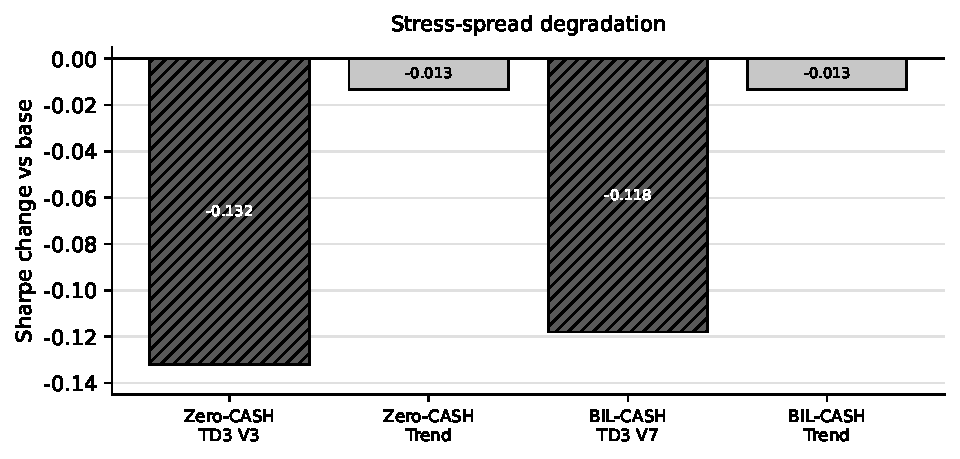
\includegraphics[width=0.82\textwidth]{figures/execution_spread_sharpe_degradation.pdf}
\caption[Stress-spread Sharpe degradation for selected TD3 candidates and Trend benchmark]{Stress-spread Sharpe degradation for selected TD3 candidates and \mbox{Trend SPY/CASH}}
\label{fig:execution-spread-sharpe-degradation}
\end{figure}

This supports the execution-sensitivity component of H5.

\subsection{Training-Budget Convergence}

Training-budget convergence checks whether the 60-episode protocol appears obviously undertrained. The convergence run covers 320 histories: four candidates, four training budgets, five seeds, and four folds, across 30, 60, 100, and 150 episodes.

The evidence does not show that 60 episodes is materially undertrained for the selected candidate-cap pairs. In the convergence output, zero rows support undertraining of the 60-episode budget; three selected candidate-cap pairs have their best Sharpe at 60 episodes, while the remaining V5 no-volatility Zero-CASH pair peaks at 30 episodes. Additional training does not improve the selected pairs and, in several cases, degrades Sharpe or increases turnover.

Figure~\ref{fig:training-budget-sharpe-convergence} plots the Sharpe path for the two benchmark-comparison TD3 candidates used in the main validation comparison. The diagnostic is consistent with the text: the 60-episode setting is not flagged as obviously undertrained for these selected pairs.

\begin{figure}[htbp]
\centering
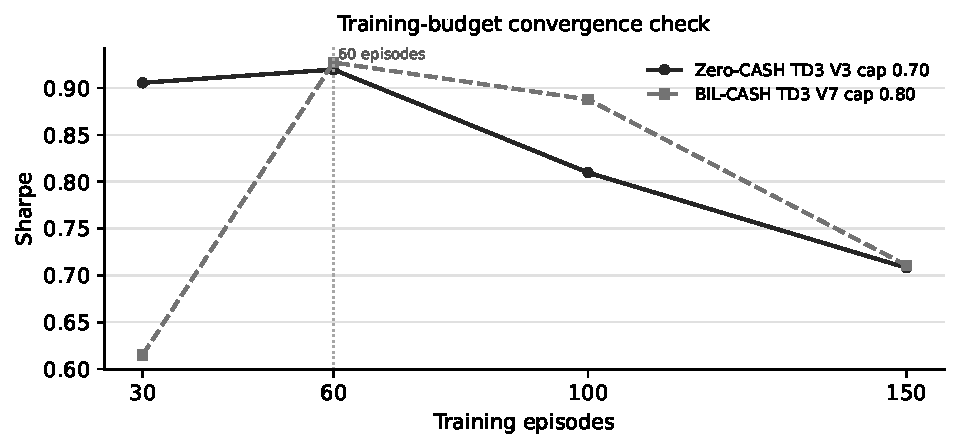
\includegraphics[width=0.82\textwidth]{figures/training_budget_sharpe_convergence.pdf}
\caption{Training-budget Sharpe convergence for selected TD3 candidates}
\label{fig:training-budget-sharpe-convergence}
\end{figure}

The convergence check is therefore interpreted as a diagnostic against obvious undertraining, not as proof of global training-budget optimality.

\subsection{Claim-versus-Evidence Summary}

The evaluation stack changes the strength of the defensible claim. Ranking competitiveness survives in a precise sense: selected DRL candidates lead relevant mandate-aware or robust diagnostic rankings, remain Pareto-competitive in several practical tradeoff views, and lead in selected regime slices.

The boundary is equally clear. Bootstrap intervals include zero and White Reality Check p-values do not support statistical superiority for the searched learning candidate. No strategy satisfies every hard mandate filter. Selected case-study histories are more sensitive to additional spread assumptions than the Trend SPY/CASH benchmark, and cash assumptions change the selected case-study candidate.

\begin{table}[htbp]
\centering
\caption{Claim versus evidence}
\scriptsize
\begin{tabularx}{\textwidth}{L{0.30\textwidth}L{0.16\textwidth}Y}
\toprule
\textbf{Claim} & \textbf{Supported?} & \textbf{Evidence} \\
\midrule
Ranking competitiveness survives. & Yes & Selected case-study candidates lead relevant diagnostic rankings, while deterministic benchmarks remain strong under standard metrics. \\
Statistical superiority is established. & No & Bootstrap confidence intervals include zero and WRC p-values do not support superiority. \\
Cash assumption matters. & Yes & Zero-CASH and BIL-CASH select different learning candidates and diagnostic-ranking leaders. \\
Execution assumptions matter. & Yes & Stress spreads degrade selected learning candidates more than Trend SPY/CASH. \\
Hard mandate feasibility is achieved. & Profile-dependent & No strategy passes the conservative hard-filter layer; moderate and aggressive feasibility remains conditional on profile and tradeoff choice. \\
Learning candidate is Pareto-competitive. & Yes & Selected case-study candidates remain on or near relevant tradeoff frontiers. \\
Benchmarks are weak. & No & Regenerated deterministic benchmarks remain strong comparators. \\
\bottomrule
\end{tabularx}
\end{table}

\newpage

\section{Conclusions, Limitations and Avenues for Further Research}

\subsection{Answer to the Research Question}

The research question asked whether a falsification-oriented evaluation framework can distinguish ranking competitiveness, statistical credibility, and practical feasibility in TD3-based cross-asset portfolio allocation. The answer is yes. The framework separates these claims and shows that they receive different levels of empirical support.

Selected TD3 candidates remain ranking-competitive under the corrected benchmark-matched framework. Bootstrap Sharpe-difference intervals and White Reality Check do not support a stronger claim of statistical superiority over clean deterministic benchmarks. Practical feasibility remains conditional on cash assumptions, hard mandate filters, Pareto tradeoffs, execution-spread stress, regime dependence, and training-budget diagnostics.

\subsection{Main Findings}

The main findings follow the claim hierarchy developed in the thesis. H1 is supported in a limited sense: selected learning candidates remain benchmark-matched ranking-competitive under the corrected protocol. H2 is also supported: statistical superiority is not established once sampling uncertainty and candidate-search bias are considered. The statistical validation layer therefore limits the strength of the claim that can be defended.

H3 is supported because cash treatment matters. Zero-CASH and BIL-CASH select different candidates and change the interpretation of allocation performance. H4 is supported because practical feasibility cannot be inferred from rankings alone; mandate constraints, Pareto tradeoffs, and investor profiles affect whether a strategy is practically relevant. H5 is supported for regime dependence, mandate constraints, and execution-spread sensitivity, while the training-budget check acts as a diagnostic boundary against obvious undertraining rather than as proof of global training-budget optimality.

The benchmark results are central to this interpretation. The benchmark set is not a collection of weak strawmen. It includes deterministic rules that capture diversification, trend following, risk-off behavior, momentum, risk parity, and classical optimization ideas. Trend SPY/CASH remains a strong comparator in both cash protocols. A learned policy must be compared against these strategies before any claim about dynamic allocation value is credible.

\subsection{Methodological Contribution}

The contribution of the thesis is a falsification-oriented evaluation framework for DRL portfolio evidence. TD3 is the case-study learner; the evaluation protocol is the contribution.

The framework turns a portfolio backtest into a structured evidence hierarchy: ranking competitiveness, statistical credibility, and practical feasibility. It combines matched benchmarks, explicit cash protocols, asset-specific costs, bootstrap Sharpe-difference intervals, White Reality Check, mandate/Pareto diagnostics, regime analysis, execution-spread stress, and training-budget convergence. The contribution is methodological rather than algorithmic: the thesis does not propose a new TD3 variant, deployable alpha, or universal superiority claim.

\subsection{Limitations}

The asset universe is compact and U.S.-centric by design. It excludes credit, real estate, broad commodities beyond gold, international equities, taxes, custody constraints, liabilities, and investor-specific withdrawal needs. BTC-USD is highly idiosyncratic and may not represent digital assets more broadly.

Execution modeling is also approximate. The protocol includes asset-specific transaction costs and an additional spread robustness layer, but it does not model full order-book depth, market impact, intraday liquidity, broker-specific routing, or tax-aware execution.

Custom mandate-aware and robust scores are diagnostic selection tools, not standalone proof. Standard metrics, hard mandate filters, Pareto analysis, bootstrap validation, and White Reality Check remain necessary to interpret results.

The evaluation uses one historical sample. Walk-forward folds and multiple seeds improve robustness, but they do not create independent market histories. The study does not include live-forward paper trading or production deployment.

Finally, the training-budget convergence check supports the use of 60 episodes for this research design, but it does not prove that the chosen budget is globally optimal. These limitations define the methodological boundaries of the evidence rather than invalidating the evaluation framework.

\subsection{Avenues for Further Research}

Further research should test the framework on broader and more international asset universes, including credit, real estate, commodities beyond gold, and non-U.S. equities. It should also examine whether the findings survive alternative market samples, live-forward paper trading, and more detailed execution modeling.

The framework can be extended to additional DRL learners, alternative reward functions, and richer state representations. Future work should also evaluate investor-specific mandates, tax-aware constraints, withdrawal needs, and capacity limits. Another extension is to replace heuristic score-like features with properly calibrated probability estimates, evaluated through out-of-sample calibration tests such as Brier scores and reliability curves. These extensions would test whether ranking competitiveness can translate into statistical credibility and practical feasibility under more demanding real-world conditions.


\newpage
\phantomsection
\addcontentsline{toc}{section}{References}
\begin{thebibliography}{99}

\bibitem[Almahdi and Yang(2017)]{almahdi2017} Almahdi, S. and Yang, S. Y. (2017). An adaptive portfolio trading system: A risk-return portfolio optimization using recurrent reinforcement learning with expected maximum drawdown. \emph{Expert Systems with Applications}, 87, 267--279.

\bibitem[Bailey and López de Prado(2014)]{bailey2014} Bailey, D. H. and López de Prado, M. (2014). The deflated Sharpe ratio: Correcting for selection bias, backtest overfitting, and non-normality. \emph{Journal of Portfolio Management}, 40(5), 94--107.

\bibitem[Binance(2026)]{binance2026tradingfees} Binance. (2026). Trading fees. \url{https://www.binance.com/es/fee/trading}. Accessed 25 June 2026.

\bibitem[Bollerslev(1986)]{bollerslev1986} Bollerslev, T. (1986). Generalized autoregressive conditional heteroskedasticity. \emph{Journal of Econometrics}, 31(3), 307--327.

\bibitem[Bouri et al.(2017)]{bouri2017bitcoinhedge} Bouri, E., Molnár, P., Azzi, G., Roubaud, D., and Hagfors, L. I. (2017). On the hedge and safe haven properties of Bitcoin: Is it really more than a diversifier? \emph{Finance Research Letters}, 20, 192--198.

\bibitem[Chen et al.(2022)]{chen2022} Chen, W., Zhang, H., and Jia, L. (2022). A novel two-stage method for well-diversified portfolio construction based on stock return prediction using machine learning. \emph{North American Journal of Economics and Finance}, 63, 101818.

\bibitem[DeMiguel et al.(2009)]{demiguel2009} DeMiguel, V., Garlappi, L., and Uppal, R. (2009). Optimal versus naive diversification: How inefficient is the 1/N portfolio strategy? \emph{Review of Financial Studies}, 22(5), 1915--1953.

\bibitem[Fujimoto et al.(2018)]{fujimoto2018} Fujimoto, S., van Hoof, H., and Meger, D. (2018). Addressing function approximation error in actor-critic methods. \emph{Proceedings of the 35th International Conference on Machine Learning}.

\bibitem[Guesmi et al.(2019)]{guesmi2019bitcoinDiversification} Guesmi, K., Saadi, S., Abid, I., and Ftiti, Z. (2019). Portfolio diversification with virtual currency: Evidence from Bitcoin. \emph{International Review of Financial Analysis}, 63, 431--437.

\bibitem[Henriques and Sadorsky(2018)]{henriques2018bitcoinGold} Henriques, I. and Sadorsky, P. (2018). Can Bitcoin replace gold in an investment portfolio? \emph{Journal of Risk and Financial Management}, 11(3), 48.

\bibitem[Hubrich(2023)]{hubrich2023bitcoin} Hubrich, S. (2023). Bitcoin in a multi-asset portfolio. \emph{Journal of Alternative Investments}, 25(3), 63--80.

\bibitem[Interactive Brokers(2026)]{interactivebrokers2026commissions} Interactive Brokers. (2026). Commissions. \url{https://www.interactivebrokers.com/es/pricing/commissions-home.php}. Accessed 25 June 2026.

\bibitem[Jagannathan and Ma(2003)]{jagannathan2003} Jagannathan, R. and Ma, T. (2003). Risk reduction in large portfolios: Why imposing the wrong constraints helps. \emph{Journal of Finance}, 58(4), 1651--1683.

\bibitem[Jegadeesh and Titman(1993)]{jegadeesh1993} Jegadeesh, N. and Titman, S. (1993). Returns to buying winners and selling losers: Implications for stock market efficiency. \emph{Journal of Finance}, 48(1), 65--91.

\bibitem[Jiang et al.(2017)]{jiang2017} Jiang, Z., Xu, D., and Liang, J. (2017). A deep reinforcement learning framework for the financial portfolio management problem. \emph{arXiv preprint arXiv:1706.10059}.

\bibitem[Jiang et al.(2024)]{jiang2024td3} Jiang, Y., Olmo, J., and Atwi, M. (2024). Deep reinforcement learning for portfolio selection. \emph{Global Finance Journal}, 62, 101016.

\bibitem[Jiang et al.(2025)]{jiang2025multiperiod} Jiang, Y., Olmo, J., and Atwi, M. (2025). Deep reinforcement learning for high-dimensional multi-period portfolio allocation. \emph{International Review of Economics and Finance}, 98, 103996.

\bibitem[Klein et al.(2018)]{klein2018bitcoin} Klein, T., Pham Thu, H., and Walther, T. (2018). Bitcoin is not the new gold: A comparison of volatility, correlation, and portfolio performance. \emph{International Review of Financial Analysis}, 58, 105--116.

\bibitem[Lillicrap et al.(2015)]{lillicrap2015} Lillicrap, T. P., Hunt, J. J., Pritzel, A., Heess, N., Erez, T., Tassa, Y., Silver, D., and Wierstra, D. (2015). Continuous control with deep reinforcement learning. \emph{arXiv preprint arXiv:1509.02971}.

\bibitem[Liu et al.(2020)]{liu2020finrl} Liu, X.-Y., Yang, H., Chen, Q., Zhang, R., Yang, L., Xiao, B., and Wang, C. D. (2020). FinRL: A deep reinforcement learning library for automated stock trading in quantitative finance. \emph{arXiv preprint arXiv:2011.09607}.

\bibitem[López de Prado(2020)]{lopezdeprado2020mlam} López de Prado, M. (2020). \emph{Machine Learning for Asset Managers}. Cambridge University Press.

\bibitem[Maillard et al.(2010)]{maillard2010} Maillard, S., Roncalli, T., and Teiletche, J. (2010). The properties of equally weighted risk contribution portfolios. \emph{Journal of Portfolio Management}, 36(4), 60--70.

\bibitem[Markowitz(1952)]{markowitz1952} Markowitz, H. (1952). Portfolio selection. \emph{Journal of Finance}, 7(1), 77--91.

\bibitem[Merton(1969)]{merton1969} Merton, R. C. (1969). Lifetime portfolio selection under uncertainty: The continuous-time case. \emph{Review of Economics and Statistics}, 51(3), 247--257.

\bibitem[Merton(1971)]{merton1971} Merton, R. C. (1971). Optimum consumption and portfolio rules in a continuous-time model. \emph{Journal of Economic Theory}, 3(4), 373--413.

\bibitem[Moody and Saffell(2001)]{moody2001} Moody, J. and Saffell, M. (2001). Learning to trade via direct reinforcement. \emph{IEEE Transactions on Neural Networks}, 12(4), 875--889.

\bibitem[Moskowitz et al.(2012)]{moskowitz2012} Moskowitz, T. J., Ooi, Y. H., and Pedersen, L. H. (2012). Time series momentum. \emph{Journal of Financial Economics}, 104(2), 228--250.

\bibitem[Novy-Marx and Velikov(2016)]{novymarx2016} Novy-Marx, R. and Velikov, M. (2016). A taxonomy of anomalies and their trading costs. \emph{Review of Financial Studies}, 29(1), 104--147.

\bibitem[Petukhina and Sprünken(2021)]{petukhina2021digitalassets} Petukhina, A. and Sprünken, E. (2021). Evaluation of multi-asset investment strategies with digital assets. \emph{Digital Finance}, 3(1), 45--79.

\bibitem[Platanakis and Urquhart(2020)]{platanakis2020bitcoin} Platanakis, E. and Urquhart, A. (2020). Should investors include Bitcoin in their portfolios? A portfolio theory approach. \emph{British Accounting Review}, 52(4), 100837.

\bibitem[Sharpe(1966)]{sharpe1966} Sharpe, W. F. (1966). Mutual fund performance. \emph{Journal of Business}, 39(1), 119--138.

\bibitem[Silver et al.(2014)]{silver2014} Silver, D., Lever, G., Heess, N., Degris, T., Wierstra, D., and Riedmiller, M. (2014). Deterministic policy gradient algorithms. \emph{Proceedings of the 31st International Conference on Machine Learning}.

\bibitem[Simutin(2014)]{simutin2014} Simutin, M. (2014). Cash holdings and mutual fund performance. \emph{Review of Finance}, 18(4), 1425--1464.

\bibitem[White(2000)]{white2000} White, H. (2000). A reality check for data snooping. \emph{Econometrica}, 68(5), 1097--1126.

\bibitem[Zhao et al.(2023)]{zhao2023correlation} Zhao, T., Ma, X., Li, X., and Zhang, C. (2023). Asset correlation based deep reinforcement learning for the portfolio selection. \emph{Expert Systems with Applications}, 221, 119707.

\end{thebibliography}

\newpage
\section*{Annexes}
\addcontentsline{toc}{section}{Annexes}
\newcommand{\annexsection}[3]{%
    \phantomsection
    \section*{Annex #1. #3}
    \addcontentsline{toc}{section}{Annex #1. #2}
    \addcontentsline{loa}{annex}{Annex #1. #2}
}

\annexsection{A}{Data and Cash Protocols}{Data, Asset Universe and Cash Protocols}

This annex records the investable universe and cash protocols used in the thesis. The universe is deliberately compact: it supports interpretable cross-asset allocation tests, not a proxy for the full global market portfolio.

\begin{table}[H]
\centering
\caption{Annex asset universe, cash protocols and transaction-cost assumptions}
\scriptsize
\begin{tabularx}{\textwidth}{L{0.16\textwidth}L{0.23\textwidth}L{0.18\textwidth}Y}
\toprule
\textbf{Sleeve} & \textbf{Proxy} & \textbf{Decision frequency} & \textbf{Cost and interpretation} \\
\midrule
Equity growth & SPY & Weekly & ETF-like transaction cost of 2 bps. \\
Duration risk & TLT & Weekly & ETF-like transaction cost of 2 bps. \\
Real safe haven & GLD & Weekly & ETF-like transaction cost of 2 bps. \\
Digital alternative risk & BTC-USD & Weekly & Crypto transaction-cost assumption of 10 bps. \\
Defensive liquidity & CASH under Zero-CASH; BIL under BIL-CASH & Weekly & CASH has zero cost under Zero-CASH. BIL is treated as ETF-like cash proxy with 2 bps under BIL-CASH. \\
\bottomrule
\end{tabularx}
\end{table}

Zero-CASH defines the defensive sleeve as a synthetic zero-return cash position. BIL-CASH replaces that synthetic assumption with BIL as a short-term Treasury ETF proxy. These protocols define different investable environments and are therefore evaluated separately.

The market-price pipeline downloads adjusted-close prices for non-synthetic assets, resamples them to weekly Friday observations, and constructs simple percentage returns. CASH is not downloaded under Zero-CASH; it is inserted as a zero-return sleeve. Under BIL-CASH, BIL returns are mapped into the CASH column while preserving the same portfolio action label. Feature matrices are aligned to the weekly return index and shifted so that features used at a decision date are available before the realized next-period return.

\begin{table}[H]
\centering
\caption{Annex data acquisition and preprocessing traceability}
\scriptsize
\begin{tabularx}{\textwidth}{L{0.28\textwidth}Y}
\toprule
\textbf{Step} & \textbf{Treatment in the project pipeline} \\
\midrule
Market prices & SPY, TLT, GLD, BTC-USD and, when required, BIL are obtained as adjusted-close price series for the configured historical window. \\
Return construction & Prices are aligned to weekly Friday observations and converted to simple percentage returns; returns are not normalized because they define realized portfolio rewards. \\
Cash treatment & Zero-CASH inserts a synthetic zero-return CASH sleeve; BIL-CASH maps BIL returns into the CASH sleeve and applies the ETF-like transaction-cost convention. \\
Missing observations & Price and return series are sorted, duplicate dates are resolved by keeping the last observation, and unusable rows with missing return values are dropped before modeling. \\
Feature timing & Features are aligned to the return index and shifted by one weekly step before training/evaluation to reduce look-ahead leakage. \\
Macro/as-of data & Macro features are built from local or FRED/ALFRED-style inputs and aligned to weekly dates; CPI availability uses a conservative lag approximation where applicable. \\
Execution scope & The experiment uses historical research data only; it does not use live trading, production execution, account-specific routing, taxes, or custody data. \\
\bottomrule
\end{tabularx}
\end{table}

The transaction-cost schedule is a transparent modeling assumption used to make turnover economically visible in the experiment. It is not an account-specific execution estimate and does not include taxes, market impact, custody fees, broker-specific routing, or investor-specific implementation constraints.

\annexsection{B}{TD3 Feature Families}{TD3 Candidate Design and Feature Families}

The TD3 search evaluates multiple state representations under one evaluation protocol. The main text keeps feature-family detail concise because the thesis evaluates the protocol, not a new feature-engineering method.

\begin{table}[H]
\centering
\caption{Annex TD3 feature families}
\scriptsize
\begin{tabularx}{\textwidth}{L{0.18\textwidth}Y Y}
\toprule
\textbf{Family} & \textbf{Role} & \textbf{Interpretation note} \\
\midrule
V2 reference & Reference financial feature set. & Baseline rich state representation. \\
V3 clean macro & Audited macro variables aligned to the allocation frequency. & Used to test whether clean macro information improves allocation evidence. \\
V4 GARCH-style volatility & Volatility-state augmentation. & Tests whether fitted volatility information changes candidate behavior. \\
V5 no-volatility representation & Volatility-block ablation. & Tests whether simpler non-volatility states remain competitive. \\
V6 financial score-like indicators & Compact financial representation. & Variables are score-like indicators, not calibrated probabilities. \\
V7 macro + GARCH & Clean macro state combined with GARCH-style volatility. & Tests whether volatility augmentation changes the clean macro specification. \\
V8 EWMA/GARCH & EWMA/GARCH volatility hybrid. & Tests an alternative volatility-state construction. \\
\bottomrule
\end{tabularx}
\end{table}

PCA was audited during the project but is not used as the default representation in the final thesis design. Full feature definitions are documented in project outputs where available; they are not expanded here to avoid turning the annex into a second methodology chapter.

\annexsection{C}{Candidate Search}{Candidate Search, Caps, Seeds and Folds}

The candidate search combines feature-family variation, max-weight caps, seeds, folds, and cash protocols. This creates a searched candidate set rather than a single fixed strategy. For that reason, the thesis separates TD3-only selection from benchmark-comparison selection and then subjects the searched set to statistical validation.

\begin{table}[H]
\centering
\caption{Annex candidate-search structure}
\scriptsize
\begin{tabularx}{\textwidth}{L{0.26\textwidth}Y}
\toprule
\textbf{Search component} & \textbf{Use in the thesis} \\
\midrule
Feature families & V2, V3, V4, V5, V6, V7 and V8 representations are evaluated as TD3 candidate designs. \\
Cap levels & Max-weight caps are searched to test whether concentration control changes policy quality and feasibility. \\
Seeds & Multiple random seeds are used to reduce reliance on a single training run. \\
Walk-forward folds & Four folds are used in the corrected protocol to evaluate out-of-sample behavior over time. \\
TD3-only selection & Identifies the strongest searched learning candidate within the TD3 universe before deterministic benchmarks are introduced. \\
Benchmark-comparison candidates & Selects learning candidates for matched comparison against regenerated deterministic benchmarks. \\
Candidate-search bias & The searched design can overstate the best observed candidate, which motivates bootstrap Sharpe-difference analysis and White Reality Check. \\
\bottomrule
\end{tabularx}
\end{table}

The searched histories share the same historical market sample and should not be interpreted as independent market histories. They are useful for stress-testing candidate behavior, but they also require caution when interpreting the strongest observed ranking.

\annexsection{D}{Benchmark Definitions}{Benchmark Definitions}

Deterministic benchmarks are regenerated under the same universe, cash assumption, cost schedule, and evaluation window as the TD3 candidates. This matching is essential: the learning candidate must be compared with clean comparators, not weak or mismatched baselines.

\begin{table}[H]
\centering
\caption{Annex benchmark families}
\scriptsize
\begin{tabularx}{\textwidth}{L{0.28\textwidth}Y}
\toprule
\textbf{Benchmark family} & \textbf{Definition in the comparison layer} \\
\midrule
Buy-and-hold sleeves & Individual buy-and-hold exposures for SPY, TLT, GLD and BTC-USD. \\
Equal-weight portfolios & Equal-weight allocation across the available sleeves, including risky-only variants where reported. \\
Static stock-bond allocation & A 60/40 SPY/TLT allocation used as a classical diversified reference. \\
Defensive risk-off rules & Rules that rotate defensively according to pre-defined risk-off logic. \\
Momentum and risk-adjusted momentum & Deterministic rotation rules based on recent performance or risk-adjusted recent performance. \\
Rolling Markowitz & Rolling long-only mean-variance allocation. \\
Rolling minimum variance & Rolling optimizer focused on variance minimization. \\
Inverse-volatility risk parity & Allocation inversely related to estimated volatility. \\
Trend SPY/CASH & Trend-following comparator that rotates between SPY and the cash sleeve. \\
\bottomrule
\end{tabularx}
\end{table}

The benchmark set is intentionally broad enough to discipline the TD3 interpretation. A favorable TD3 ranking is meaningful only after these deterministic references are evaluated under matching assumptions.

\annexsection{E}{Statistical Validation}{Statistical Validation Details}

The statistical validation layer separates ranking competitiveness from statistical superiority. The pairwise bootstrap Sharpe-difference procedure estimates uncertainty around the Sharpe difference between a selected TD3 candidate and the clean benchmark comparator. If the interval includes zero, the ranking advantage is not interpreted as reliable statistical superiority.

White Reality Check is used as search-adjusted candidate-set evidence. In plain technical language, the null hypothesis is that the searched TD3 candidate set does not provide superior performance relative to the benchmark comparator once data-snooping across candidates is considered. The candidate set is defined by the searched TD3 policies in the corrected evaluation layer. The comparator logic uses the clean deterministic benchmark selected for statistical comparison, especially Trend SPY/CASH in the reported validation.

\begin{table}[H]
\centering
\caption{Annex interpretation of statistical validation outputs}
\scriptsize
\begin{tabularx}{\textwidth}{L{0.27\textwidth}Y}
\toprule
\textbf{Output} & \textbf{Interpretation} \\
\midrule
Bootstrap Sharpe difference & Pairwise uncertainty around the Sharpe difference between a selected TD3 candidate and the benchmark comparator. \\
Confidence interval crossing zero & The evidence does not support a statistical superiority claim for the displayed pair. \\
White Reality Check p-value & Search-adjusted evidence for the searched candidate set against the comparator. \\
High WRC p-value & The candidate-set evidence is not strong enough to reject the data-snooping-adjusted null. \\
Limitation & Statistical tests reduce overstatement, but they do not create independent market histories or live-forward evidence. \\
\bottomrule
\end{tabularx}
\end{table}

These tests are guardrails. They do not invalidate ranking competitiveness, but they prevent a ranking result from being converted into a stronger alpha or superiority claim.

\annexsection{F}{Regime and Feasibility Diagnostics}{Regime, Mandate and Pareto Diagnostics}

The regime, mandate and Pareto diagnostics evaluate whether selected strategies remain interpretable under market-state variation and practical constraints. They are diagnostic tools, not standalone proof of superiority.

\begin{table}[H]
\centering
\caption{Annex regime and feasibility diagnostics}
\scriptsize
\begin{tabularx}{\textwidth}{L{0.24\textwidth}Y}
\toprule
\textbf{Diagnostic} & \textbf{Role in interpretation} \\
\midrule
Regime categories & COVID shock/recovery, inflation and hiking shocks, post-COVID liquidity, AI/risk-on expansion, recent test windows, and calendar-year regimes. \\
Mandate profiles & Conservative, moderate and aggressive profiles are used to evaluate investor-relevant suitability. \\
Hard mandate filters & Hard constraints provide pass/fail feasibility checks rather than smooth ranking scores. \\
Pareto tradeoffs & Pareto analysis evaluates return, risk, drawdown, turnover, concentration and related tradeoffs without requiring one scalar winner. \\
Diagnostic scores & Mandate-aware and robust scores support selection diagnostics, but they are not standalone proof of statistical superiority or deployability. \\
\bottomrule
\end{tabularx}
\end{table}

The practical interpretation is conservative. A candidate may be ranking-competitive while still failing hard mandate filters, depending on a cash assumption, or occupying a tradeoff frontier rather than dominating all metrics.

\begin{table}[H]
\centering
\caption{Annex hard mandate-filter thresholds}
\scriptsize
\begin{tabularx}{\textwidth}{L{0.20\textwidth}rrrrY}
\toprule
\textbf{Profile} & \textbf{Max DD} & \textbf{Max ann. vol.} & \textbf{Min eff. assets} & \textbf{Max avg. turnover} & \textbf{Interpretation} \\
\midrule
Conservative & -0.10 & 0.10 & 3.00 & 0.05 & Tight drawdown, volatility, diversification, and implementation-discipline limits. \\
Moderate & -0.15 & 0.15 & 2.30 & 0.10 & Balanced drawdown, volatility, diversification, and turnover limits. \\
Aggressive & -0.25 & 0.25 & 1.50 & 0.20 & Looser risk, diversification, and turnover limits for higher-risk profiles. \\
\bottomrule
\end{tabularx}
\vspace{2pt}
\parbox{\textwidth}{\scriptsize\textit{Note: Max-weight caps are structural TD3 experiment constraints, not official mandate-filter thresholds. Concentration is represented here by the effective-assets minimum.}}
\end{table}

\annexsection{G}{Execution and Training Diagnostics}{Execution-Spread Stress and\\Training-Budget Convergence}

Execution-spread stress is post-training and reporting-only. It does not retrain TD3, does not alter the original training objective, and does not create new final winners. Its role is to test whether selected reported histories remain economically interpretable under less favorable execution assumptions.

Training-budget convergence evaluates whether the 60-episode protocol appears obviously undertrained for the selected candidate-cap pairs. The check compares 30, 60, 100 and 150 episodes. It is interpreted as a diagnostic against obvious undertraining, not as proof that the training budget is globally optimal.

\begin{table}[H]
\centering
\caption{Annex robustness-check boundaries}
\scriptsize
\begin{tabularx}{\textwidth}{L{0.30\textwidth}Y}
\toprule
\textbf{Check} & \textbf{Boundary of the claim} \\
\midrule
Execution-spread stress & Reporting-only sensitivity analysis after training; it does not select new winners or retrain policies. \\
Training-budget convergence & Checks 30, 60, 100 and 150 episodes for obvious undertraining; it does not prove global training-budget optimality. \\
Interpretation & Both checks affect practical interpretation, but neither converts ranking competitiveness into statistical superiority. \\
\bottomrule
\end{tabularx}
\end{table}

\annexsection{H}{Reproducibility Artifacts}{Reproducibility and Project Outputs}

This annex lists the main reproducibility artifacts supporting the thesis. The paths refer to the project folder used for the empirical work.

\begin{table}[H]
\centering
\caption{Annex reproducibility artifacts}
\scriptsize
\begin{tabularx}{\textwidth}{L{0.27\textwidth}Y}
\toprule
\textbf{Artifact type} & \textbf{Known project files or folders} \\
\midrule
Project root & Repository root for the thesis project; paths below are relative to this root. \\
Repository access & Available upon request. \\
Data preparation scripts & \path{src/data/build_dataset.py}; \path{src/data/build_macro_dataset.py}; \path{src/data/build_realtime_macro_dataset.py}; \path{src/data/prepare_dataset.py} \\
TD3 training scripts & \path{src/train/train_td3.py}; \path{src/models/td3_agent.py}; \path{src/models/actor.py}; \path{src/models/critic.py} \\
Benchmark scripts & \path{src/backtest/benchmarks.py}; \path{src/backtest/dynamic_allocation_benchmarks.py}; \path{src/backtest/performance_metrics.py} \\
Statistical validation scripts & \path{src/analysis/statistical_validation_report.py}; \path{src/analysis/white_reality_check_report.py} \\
Robustness scripts & \path{src/analysis/regime_analysis_report.py}; \path{src/analysis/mandate_profile_comparison_report.py}; \path{src/analysis/asset_specific_constraint_pareto_report.py}; \path{src/analysis/execution_spread_robustness_report.py}; \path{src/analysis/training_budget_convergence_report.py} \\
Output tables & \path{outputs/tables/asset_specific_cost_full_final_report/}; \path{outputs/tables/asset_specific_cost_benchmark_comparison/}; \path{outputs/tables/asset_specific_cost_statistical_validation/}; \path{outputs/tables/asset_specific_cost_white_reality_check/}; \path{outputs/tables/asset_specific_cost_regime_analysis/}; \path{outputs/tables/asset_specific_cost_constraint_pareto/}; \path{outputs/tables/asset_specific_cost_mandate_profile_comparison/} \\
Generated thesis source & \path{tfm/main.tex}; \path{tfm/main.pdf} \\
\bottomrule
\end{tabularx}
\end{table}

\annexsection{I}{Core Implementation Logic}{Core Implementation Logic}

This annex records the implementation logic needed to reproduce the main empirical interpretation. It is intentionally compact: the authoritative implementation remains in the project files listed in Annex H, while the blocks below document the portfolio mechanics, matched evaluation protocol, and statistical validation workflow used to interpret the evidence.

\textbf{Procedure 1. Feasible action, cost, net return, and reward logic}

\begin{enumerate}[label=\arabic*.,leftmargin=*,itemsep=2pt,parsep=0pt,topsep=4pt]
    \item Receive the raw action $a_t$ from the deterministic policy, the previous drifted portfolio weights, next-period asset returns, and asset-specific transaction-cost rates.
    \item Project $a_t$ onto the long-only simplex to obtain the executed feasible weights $w_t$.
    \item Compute asset-level turnover as the absolute difference between executed weights and previous drifted weights.
    \item Compute transaction-cost drag as the turnover-weighted sum of asset-specific cost rates.
    \item Compute gross portfolio return from $w_t$ and next-period asset returns.
    \item Compute net portfolio return by subtracting transaction-cost drag from gross return.
    \item Update portfolio value, running peak, and drawdown.
    \item Compute the reward as net return adjusted by the configured drawdown penalty.
    \item Store the transition using feasible weights and the net-return-based reward.
\end{enumerate}

\textbf{Procedure 2. Walk-forward and benchmark-matched evaluation protocol}

\begin{enumerate}[label=\arabic*.,leftmargin=*,itemsep=2pt,parsep=0pt,topsep=4pt]
    \item For each cash protocol, build the same investable universe, cost assumptions, and date windows.
    \item For each walk-forward split, train candidate TD3 policies only on the training window.
    \item Select candidates using the predefined diagnostic score stack.
    \item Evaluate selected candidates out-of-sample without exploration noise.
    \item Regenerate deterministic benchmarks under the same asset universe, cash protocol, transaction-cost convention, rebalance frequency, and train/test window.
    \item Aggregate out-of-sample results by candidate, cap, seed, and split.
    \item Interpret TD3 only against matched benchmark evidence.
\end{enumerate}

\textbf{Procedure 3. Statistical validation workflow}

\begin{enumerate}[label=\arabic*.,leftmargin=*]
    \item Build the searched TD3 candidate set from the final evaluation outputs.
    \item For each selected TD3 candidate and clean benchmark comparator, compute paired out-of-sample return differentials.
    \item Estimate the Sharpe-difference statistic for the selected comparison.
    \item Bootstrap paired return histories to obtain the confidence interval for the Sharpe difference and the probability that the selected TD3 candidate beats the comparator.
    \item Across the searched candidate set, apply White Reality Check to candidate return differentials.
    \item Report the search-adjusted p-value.
    \item Interpret ranking competitiveness only when rankings support it; do not claim statistical superiority when intervals include zero or White Reality Check does not reject the null.
\end{enumerate}

\begin{flushleft}
The corresponding source areas are \path{src/env/portfolio_env.py}, \path{src/utils/action_projection.py}, \path{src/backtest/}, and \path{src/analysis/}. Relative project paths are reported to make the implementation traceable across computing environments and to support independent reproducibility.
\end{flushleft}

% Manual verification needed: confirm whether the university has a newer official MECOFIN Word template, because the supplied .doc file resolves locally as an HTML 404 page rather than a usable template file.

\end{document}
